% 第 2 章
\section{一维线性回归：一条直线里的相关性、方向与因果}\label{sec:onedim}

从最简模型出发——没有截距、只有一个特征：
\begin{equation}\label{eq:1d-model}
  y_i = b\, x_i + \varepsilon_i, \qquad i = 1, \dots, n,
\end{equation}
其中 $b \in \R$ 是待估参数。这一章做两件事：先\textit{从回归的角度}看 $b$ 如何度量 $x$ 与 $y$ 的相关性；再\textit{从方差的角度}看同一条直线如何暴露相关性的\textit{方向性}，以及为什么它不能告诉你因果。

\subsection{最小二乘：把均值推广成一条线}\label{sec:1d-ls}

先忘记统计。把拟合问题写成优化问题：找 $b$，让残差平方和
\begin{equation}\label{eq:1d-rss}
  S(b) = \sum_{i=1}^n (y_i - b\, x_i)^2
\end{equation}
最小。对 $b$ 求导并令其为零：
\[
  \frac{dS}{db} = -2 \sum_{i=1}^n x_i (y_i - b x_i) = 0
  \quad\Longrightarrow\quad
  \boxed{\;\hat{b} = \frac{\sum_{i=1}^n x_i y_i}{\sum_{i=1}^n x_i^2}\;}
\]
二阶导数 $\frac{d^2 S}{db^2} = 2 \sum_i x_i^2 > 0$（只要 $x$ 不全为零），故这是唯一的全局最小值点。没有初值、没有学习率、没有局部极小值——凸性一次性解决。

先看两个极端，建立直觉。若 $x_i \equiv 1$，$\hat{b} = \bar{y}$：\textbf{最小二乘是均值的推广}，样本均值正是使平方偏差最小的那个常数。若模型有截距 $y_i = a + b x_i + \varepsilon_i$，完全一样的求导给出
\begin{equation}\label{eq:1d-slope}
  \hat{b} = \frac{\Cov_n(x, y)}{\Var_n(x)}, \qquad \hat{a} = \bar{y} - \hat{b}\,\bar{x},
\end{equation}
即回归线必过数据中心点 $(\bar{x}, \bar{y})$。请把 \eqref{eq:1d-slope} 慢慢读一遍：\textit{斜率 = $x$ 与 $y$ 一起变化的程度，除以 $x$ 自身变化的程度}。整个应用统计学中被引用最多的公式，不过是一次求导的结果。注意此时还没有假设任何误差分布——最小二乘到目前为止纯粹是几何优化。

\subsection{回归视角：斜率就是相关系数}\label{sec:1d-corr}

现在把数据标准化。记 $\sigma_x = \sqrt{\Var_n(x)}$，$\sigma_y = \sqrt{\Var_n(y)}$，Pearson（1896）相关系数\cite{pearson1896}为
\begin{equation}\label{eq:rho}
  r = \frac{\Cov_n(x, y)}{\sigma_x \, \sigma_y} \in [-1, 1].
\end{equation}
（由 Cauchy--Schwarz 不等式 $|\Cov_n(x,y)| \le \sigma_x \sigma_y$ 可知 $r$ 确实落在 $[-1,1]$。）代入 \eqref{eq:1d-slope}：
\begin{equation}\label{eq:slope-rho}
  \boxed{\;\hat{b} = r \, \frac{\sigma_y}{\sigma_x}\;}
\end{equation}

这一行是全章的枢纽，它说三件事：

\begin{enumerate}[label=(\arabic*)]
  \item \textbf{相关的\textit{强度}}（$|r|$，无量纲、对称、与单位无关）决定回归线的\textit{陡度}（以标准差为单位）：$\frac{\hat{b}\, \sigma_x}{\sigma_y} = r$。把 $x$ 移动一个标准差，预测 $\hat{y}$ 移动 $r$ 个标准差。
  \item \textbf{$r$ 的对称性 vs.\ 回归的方向性}：$r$ 对换 $x$、$y$ 不变；但回归线 $y \sim x$（以 $x$ 预测 $y$）与回归线 $x \sim y$ 是两条\textit{不同}的线（见 \ref{sec:1d-direction} 节）。
  \item \textbf{拟合优度}：判定系数
  \begin{equation}\label{eq:r2-rho2}
    R^2 = 1 - \frac{\sum_i e_i^2}{\sum_i (y_i - \bar{y})^2} = r^2,
  \end{equation}
  即「$y$ 的样本方差中被 $x$ 线性解释的比例」恰好是相关系数的平方。$R^2$ 度量相关性，而 $r$ 还带有符号（方向）。
\end{enumerate}

\begin{example}[Galton 的身高回归]\label{ex:galton}
Galton（1886）研究 205 对父母与 928 名成年子女的身高，以「中亲身高」$x$ 预测子代身高 $y$，得到的回归方程约为 $y = 0.516\,x + 33.73$（英寸）\cite{galton1886}。两代人的标准差几乎相同（约 3.3 英寸），于是以标准差计的斜率就是 $r \approx 0.5$：父母比平均值高一个标准差，子女平均只高半个标准差。高个父母的子女\textbf{趋向平庸}，矮个父母的子女同样趋向平庸——「回归均值」（regression toward the mean）由此得名。这不是生物学的规律，是 \eqref{eq:slope-rho} 的算术：只要 $|r| < 1$ 且两变量各自散布稳定，极端必然后退。\end{example}

\begin{remark}
「回归均值」是统计误用之祖：体育画报魔咒、第二次考试退步、《商业平庸的胜利》（Secrist, 1933）之流的「论证」，本质都是把噪声当作了规律。Galton 本人则用更精细的论证避开了这个陷阱\cite{galton1886,stigler1986}。
\end{remark}

\begin{figure}[htbp]
  \centering
  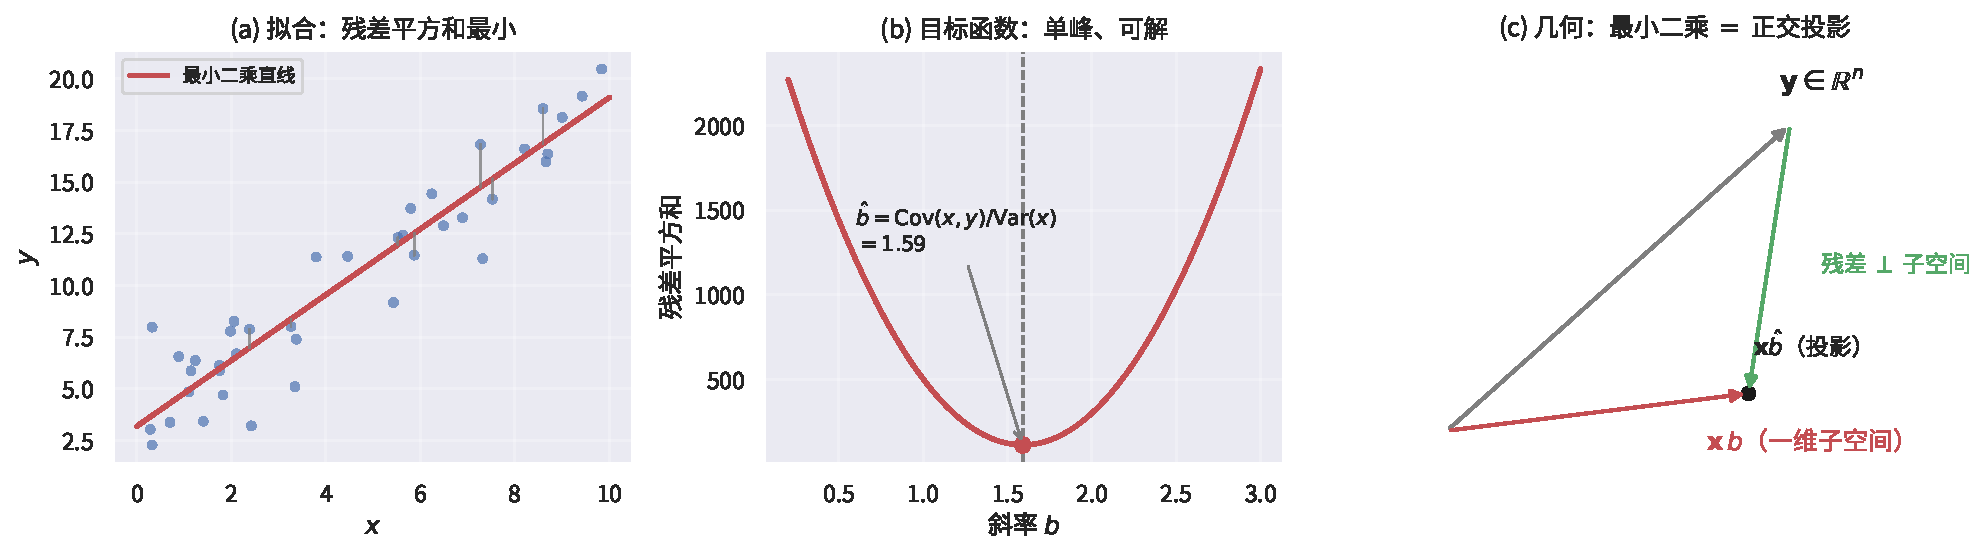
\includegraphics[width=\linewidth]{figures/ch2_leastsq.pdf}
  \caption{一维最小二乘的三个侧面：(a) 拟合——残差（竖线）平方和最小；(b) 优化——目标函数对斜率 $b$ 单峰，$\hat b=\Cov(x,y)/\Var(x)$ 可一步解出；(c) 几何——$\x\hat b$ 是 $\y$ 在一维子空间上的正交投影，残差 $\perp$ 子空间。}
  \label{fig:ch2-leastsq}
\end{figure}

\subsection{方差视角：相关从哪里来，又意味着什么}\label{sec:1d-var}

换一种眼光。把 \eqref{eq:1d-model} 中的 $y$ 看成随机变量 $y = bx + \varepsilon$，假设 $\Cov(x, \varepsilon) = 0$（即 $x$ 中不含 $y$ 的噪声成分——这本身就是一个方向性假设！）。方差的代数给出
\begin{equation}\label{eq:var-decomp}
  \Var(y) = b^2 \Var(x) + \Var(\varepsilon).
\end{equation}
\textbf{$y$ 的波动被拆成两部分：由 $x$ 携带的部分 $b^2\Var(x)$，和无法归约的噪声 $\Var(\varepsilon)$。}立刻得到
\begin{equation}\label{eq:r2-var}
  R^2 = \frac{b^2 \Var(x)}{\Var(y)} = 1 - \frac{\Var(\varepsilon)}{\Var(y)},
\end{equation}
与 \eqref{eq:r2-rho2} 殊途同归：$r^2$ 既是「样本层面拟合优度」，又是「总体层面被解释的方差占比」。这就是用方差视角看回归的第一个收获——\textit{相关性的实质，是方差的转移}。

第二个收获更深。\eqref{eq:var-decomp} 里 $b$ 的方向（正负）描述的是「$x$ 的波动如何翻译成 $y$ 的波动」。若真实结构其实是 $y$ 导致 $x$，仍按 $y \sim x$ 回归，得到的仍是同一个 $\hat{b} \approx r\,\sigma_y/\sigma_x$。相关性对生成方向\textit{完全盲视}——这是下一节的主旨。

\subsection{方向性：两条回归线，与一条主轴}\label{sec:1d-direction}

把 $x$、$y$ 都标准化（均值为 0、方差为 1），则两个方向的\textbf{回归系数}都等于 $r$：
\[
  \text{回归 } y \sim x \text{ 的系数} = r,
  \qquad
  \text{回归 } x \sim y \text{ 的系数} = r,
  \qquad
  \text{两系数之积} = r^2 < 1 \; (|r| < 1).
\]
（第二个等号是「系数」而非「斜率」：$x \sim y$ 回归解出的是 $x = r\,y$，把 $y$ 当自变量读，系数确实是 $r$。）也就是说，除非 $|r| = 1$（完全线性，无噪声），\textbf{「用 $x$ 预测 $y$ 的线」与「用 $y$ 预测 $x$ 的线」是两条不同的直线}。这里有一个必须说清的口径问题：\textit{回归系数}与\textit{画在同一坐标系里的几何斜率}不是一回事。原始尺度上两条线的回归系数分别是
\[
  b = r\,\frac{\sigma_y}{\sigma_x} \;(y \sim x), \qquad
  b' = r\,\frac{\sigma_x}{\sigma_y} \;(x \sim y),
  \qquad b\, b' = r^2 < 1,
\]
——系数之积是 $r^2$，这是 Galton「回归均值」的算术；但若把两条线都画在「$x$ 横轴、$y$ 纵轴」的同一坐标系里，第二条线要改写成 $y = \dfrac{\sigma_y}{r\,\sigma_x}\,x$，\textbf{几何斜率}分别为 $r\,\sigma_y/\sigma_x$ 与 $\sigma_y/(r\,\sigma_x)$，乘积恒为 $1$。两个乘积都对，只是度量了两个不同的问题：前者问「两个方向的预测各收缩多少」，后者问「两条直线在图上的张角」。点云近似一个椭圆（二元正态的样子），两条回归线分别是：竖直残差最小的线与水平残差最小的线——都不是椭圆的主轴（主轴对应 PCA，要求\textit{垂直}距离最小）。把图 \ref{fig:ellipse} 看进脑子里，「回归有方向、相关没有」就不再是口号。

\begin{figure}[htbp]
\centering
\resizebox{0.72\linewidth}{!}{%
\begin{tikzpicture}[>=Stealth, scale=2.6]
  % 点云椭圆
  \draw[thick, color=black!60, rotate around={35:(0,0)}] (0,0) ellipse (2.2 and 1.0);
  \fill[black!40] (35:1.3) circle (0.02);
  \fill[black!40] (215:0.9) circle (0.02);
  \fill[black!40] (35:-0.8) circle (0.02);
  \fill[black!40] (215:1.6) circle (0.02);
  \fill[black!40] (35:0.3) circle (0.02);
  \fill[black!40] (215:-1.4) circle (0.02);
  \draw[->] (-2.9,0) -- (2.9,0) node[below left] {$x$};
  \draw[->] (0,-2.3) -- (0,2.3) node[below left] {$y$};
  % 主轴
  \draw[thick, dashed, color=black!50] (-2.35,-1.65) -- (2.35,1.65) node[above right=-2pt] {主轴（PCA）};
  % 回归线 y~x: 斜率 tan(35°) * (短轴/长轴) ≈ 0.7*0.455 ≈ 0.32 → 用 rotate 近似
  \draw[very thick, color=accent] (-2.7,-0.86) -- (2.7,0.86) node[below right=-2pt] {回归 $y \sim x$};
  % 回归线 x~y
  \draw[very thick, color=red!70!black] (-1.35,-2.2) -- (1.35,2.2) node[above=-2pt] {回归 $x \sim y$};
\end{tikzpicture}}
\caption{标准化后的二元正态点云（椭圆）。两条回归线都不重合于主轴：$y \sim x$ 最小化竖直残差，$x \sim y$ 最小化水平残差，主轴最小化垂直残差。回归是\textit{有方向}的运算，相关系数 $r$ 则没有。}
\label{fig:ellipse}
\end{figure}

方向性还有一个纯代数的表述：\eqref{eq:var-decomp} 的分解 $\Var(y) = b^2\Var(x) + \Var(\varepsilon)$ 与 $\Var(x) = \tilde{b}^2 \Var(y) + \Var(\tilde\varepsilon)$（$x$ 对 $y$ 回归）可以同时成立，且各自的 $R^2$ 都是 $r^2$。两个方向「解释力」相同，这正是相关性对称性的方差表达；而斜率不同，则是方向性的表达。

\subsection{因果性：相关系数永远给不出的东西}\label{sec:1d-causality}

为什么 $r$ 不能断言因果？因为至少三种截然不同的生成机制，产生\textit{完全相同}的相关系数：

\begin{center}
\begin{tabular}{@{}lll@{}}
\toprule
结构 & 生成方式 & 观测到的相关 \\
\midrule
$x$ 导致 $y$ & $y = bx + \varepsilon$ & $r \neq 0$ \\
$y$ 导致 $x$ & $x = \tilde{b} y + \tilde\varepsilon$ & $r \neq 0$（同一个 $r$） \\
共同原因 $z$ & $x = c z + u,\;\; y = d z + v$ & $r = \mathrm{sign}(cd)\cdot(\text{由 } c,d \text{ 决定})$ \\
\bottomrule
\end{tabular}
\end{center}

数据本身对这三种情形零区分能力——这是 Reichenbach（1956）\textbf{共同原因原理}的推论：若 $A$、$B$ 统计相关，则要么 $A$ 导致 $B$，要么 $B$ 导致 $A$，要么存在共同原因 $C$\cite{reichenbach1956}。原理给出了枚举，却没有给出判别——判别必须借助数据之外的知识。

Wright（1921）是第一个把这件事做成演算的人\cite{wright1921}。他的\textbf{路径分析}说：在一张给定的因果图（箭头必须从实验、时序或领域知识中事先画出）上，任意两变量的相关系数等于连接它们的所有合法路径上系数乘积之和。于是：
\begin{itemize}
  \item \textit{正向使用}：给定因果假设，用观测到的相关去\textit{检验}它（拟合、残差相关应为零）；
  \item \textit{反向使用}：从相关反推因果结构，统计学本身无能为力——「这些结论的正确性取决于方法之外的知识」（Wright 原文的意思\cite{wright1921}）。
\end{itemize}

一百多年过去了，这个判据依然是全部因果推断（结构方程模型、DAG、do-演算、双重差分、工具变量）的根基：\textbf{回归输出的是条件关联，把系数读成因果效应需要识别策略}——随机化、自然实验、或不可检验的「无未测混杂」假设。这条界限不在任何 $t$ 统计量的射程之内。

\begin{keybox}[本章要点]
\begin{itemize}
  \item 一维最小二乘斜率 $\hat{b} = \Cov_n(x,y)/\Var_n(x) = r\,\sigma_y/\sigma_x$：回归是均值的推广，相关系数是它的标准化形态，$R^2 = r^2$ 同时是拟合优度与被解释方差占比。
  \item 方差视角：$\Var(y) = b^2\Var(x) + \Var(\varepsilon)$，相关性即方差的转移；$\Cov(x,\varepsilon)=0$ 已经是方向性假设。
  \item 方向性：$y \sim x$ 与 $x \sim y$ 是两条不同的回归线（回归系数之积为 $r^2$，画在同一坐标系里的几何斜率之积恒为 $1$）；相关系数对称，回归不对称。
  \item 因果性：至少三种结构产生同一个 $r$；共同原因原理给出枚举，路径分析给出「有外部因果知识时的演算」，但数据本身永远无法判定方向。
\end{itemize}
\end{keybox}
